\section{Introduction}

Version control is a system that records changes to a file or set of files over
time so that you can recall specific versions later. Git is a Distributed
Version Control System (VCS). In a DVCS, clients don't just check out the
latest snapshot of the files; rather, they fully mirror the repository,
including its full history.~\cite{chacon}

The major difference between Git and any other VCS is the way Git thinks about
its data. Conceptually, most othe systems store information as a list of
file-based changes. Git thinks of its data more like a series of snapshots of a
miniature filesystem. With Git, every time you commit, or save the state of your
project, Git basically takes a picture of what all your files look like at that
moment and stores a reference to that snapshot. To be efficient, if files have
not changed, Git doesn't store the file again, just a link to the previous
identical file it has already stored.~\cite{chacon}

\begin{figure}[H]
\centering
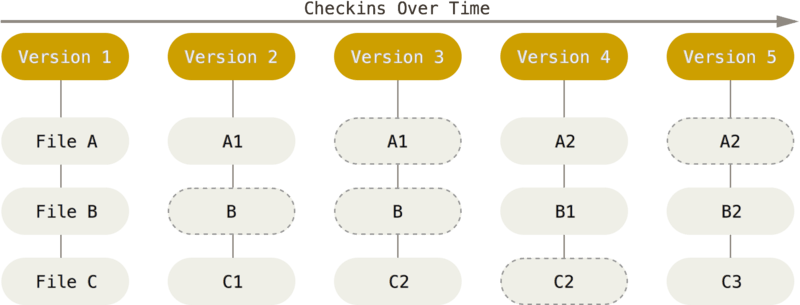
\includegraphics[width=0.75\textwidth]{snapshots.png}
\caption{Storing data as snapshots over time.}
\end{figure}

Everything in Git is checksummed before it is stored and is then referred to by that checksum.
For checksumming, Git uses a SHA-1 hash.

Git has three main states in which files can reside in:

\begin{itemize}
  \item \textbf{committed}: means that the data is safely stored in the local
  database.
  \item \textbf{modified}: means that a file has changed, but it have not
  been committed to the local database yet.
  \item \textbf{staged}: means that a modified file has been marked in its
  current version to go into the next commit snapshot.
\end{itemize}

\begin{figure}[H]
\centering
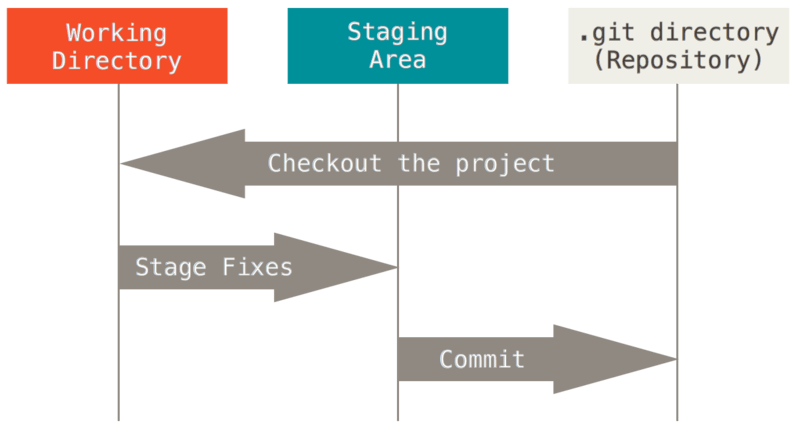
\includegraphics[width=0.75\textwidth]{areas.png}
\caption{Main states: working tree, staging area, and Git directory.}
\end{figure}

A basic Git workflow goes something like this:

\begin{enumerate}
  \item A file in working tree is modified.
  \item The modified file is staged.
  \item The staged changes are committed, which takes the files as they are in
  the staging area and stores that snapshot permanently.
\end{enumerate}

Git stores all its content as tree and blob objects. Trees correspond to UNIX
directory entries and blobs correspond to file contents. A single tree object contains
one or more entries, each of which is the SHA-1 hash of a blob or subtree with its
associated mode and filename.

\begin{figure}[H]
\centering
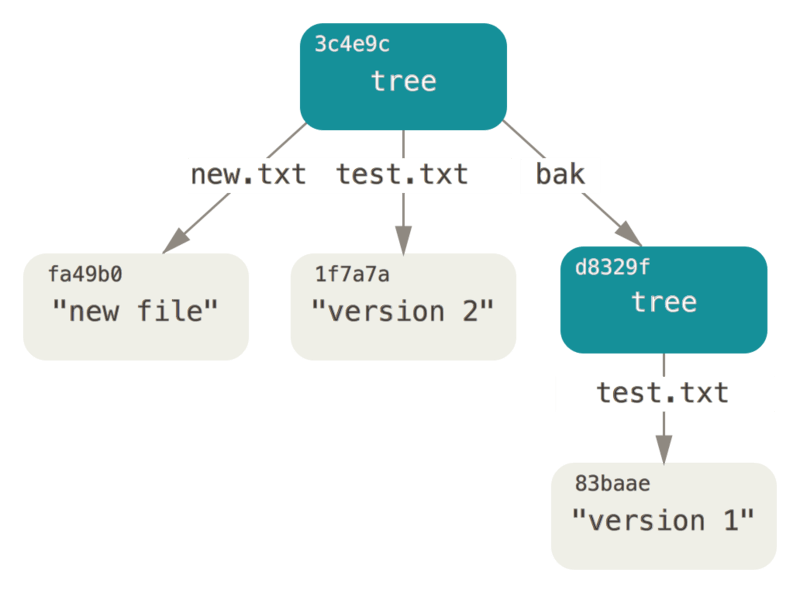
\includegraphics[width=0.75\textwidth]{data-model.png}
\caption{Git data model.}
\end{figure}

\newpage
